\documentclass[9pt]{article}
\usepackage{amsthm, amsmath, extsizes, multicol, enumitem, graphicx, wrapfig}
\usepackage[margin=0.25in]{geometry}
\usepackage[normalem]{ulem}
\begin{document}
\graphicspath{ {final_img/} }
\setlength{\multicolsep}{2pt}
\noindent\uline{\textbf{Chapter 1}}\newline
\uline{Finite Automata} $(Q - $states, $\Sigma - $alphabet, $ \delta - $transitions,
$q_0 - $start, $F\subset Q - $accept$)$. Language is \textbf{regular} if a finite 
automaton recognizes it. Two machines are equivalent if they recognize the same
language.
\begin{itemize}[noitemsep, topsep=0pt]
    \item[-]\uline{Derterministic (DFA)} Restrict to one transition for each unique 
    symbol.
    \item[-]\uline{Nondeterministic (NFA)} Every NFA has an equivalent DFA and any 
    DFA is a valid NFA. Therefore a language is \textbf{regular} if and only if some 
    NFA recognizes it. 
    \item[-]\uline{DFA to NFA} Start at start state(s). Follow and write next possible 
    states per symbol. Create new row for resulting states. Repeat until no new states.
    Should be 1 more state than the NFA.
    \item[-]\uline{Generalized nondeterministic finite automaton (GNFA)} Only one start
    and reject state. Transitions are regular expressions. Used to convert DFA to a RE.
    \item[-]\uline{DFA to DE} Add new start state and accept state. Transition start 
    to old start and from old accept to new accept. Identify destination states from 
    the state that will be removed. Identify all paths destination states have that go
    through the state that will be removed. Write new transitions excluding the removed
    state. Repeat.
\end{itemize}
\uline{Regular Languages} are closed under \textbf{union, intersection, complement, 
concatenation, star (*)}. All finite languages are Regular Languages. \newline
\uline{Power Set} is the set of all subsets of a language. Size of $P(A) = 2^{|A|}$. 
\newline
\uline{Regular Expression}. R is a RE if it is (1) a character in the alphabet 
associated with R. (2) the empty string. (3) the empty language. (4) two regular 
languages under union. (5) two regular languages under concatenation. (6) a regular 
language under star. \textbf{Order of Operations} is parenthesis, star, concatenation,
union. A language described by a RE is \textbf{regular}.\newline
\uline{Pumping Lemma for RL} A string of length at least pumping-length can be broken
up into $xyz$ such that (1) $xy^iz$ is in the language for any $i\geq 0$. (2) $|y|>0$
(3) $|xy| \leq p$.\newline
\uline{Finite Automata Theorems} For a finite automata $M$ with $n$ states (1) $L(M)$ 
is non-empty if and only if $M$ accepts a string of length less than $n$ (2) $L(M)$ is 
infinite if and only if $M$ accepts a string of length $i$ where $n\leq i < 2n$. It is
possible to create a FA that can determine if two FA are equivalent and taking a 
finite amount of time if they are equivalent.\newline
\noindent\uline{\textbf{Chapter 2}}\newline
\uline{Context-free Grammar} ($V-$variables (states), $\Sigma-$terminals (symbols), 
$R-$rules (transitions), $S-$start). Parse-trees show the path the CFG takes to output
the string. Any language made by a CFG is a \textbf{context-free} language. A CFG is
\textbf{ambiguous} if there is more than one way to generate a string (two parse trees). 
A CFL is \textbf{inherently ambiguous} if all grammars for the language are ambiguous. 
\textbf{Leftmost} deviation means the leftmost remaining variable is the one replaced; 
same for rightmost.\newline
\uline{Context-free Languages} are closed under \textbf{union, concatenation, star (*)}. 
All Regular languages are context-free.\newline
\uline{Chomsky Normal Form} if every rule is of the form $A\rightarrow BC$ or 
$A\rightarrow a$. The start variable can have a $\epsilon$. (1) Add new start variable 
with rule to old start variable. (2) Eliminate all $\epsilon$ rules. (3) Eliminate all
unit rules. (3) Convert remaining to proper form by moving stuff around. Any CFL can be 
generated by a CFG in Chomsky normal form.\newline
\uline{Pushdown Automata (PDA)} Same setup as a FA, except the inclusion of a stack
and the transitions that can pop or push something on the stack. A language is 
\textbf{context-free} if and only if some PDA recognizes it. Every regular language is
context-free.\newline
\uline{Pumping Lemma for CFL} If L is a CFL, then there is a pumping-length where if
a string in L is at least pumping-length then the string can be broken up into $uvxyz$
where (1) $uv^ixy^iz \in L$ for all $i\geq 0$. (2) $|xy|>0$ (3) $|vxy|\geq p$\newline
\uline{\textbf{Examples}}\newline
\uline{Prove $\{0^n1^m0^n \mid m,n \geq 0\}$ is not regular.} Assume this language 
($A$) is regular, so then there must exist a variable $p$, the pumping length. Choose 
$w = 0^p10^p$ as the test word. $|w|>p$ and $w\in A$. As $|xy|\leq p$, $x$ and $y$ must 
be composed of only zeros. Additionally, as $|y|>0$, $y$ would then have to equal $0^k$ 
for some $k>0$. For $xy^iz$, choose $i=0$ and the resulting word should still be in $A$. 
However $xy^0z=xz = 0^{p-k}10^p$. This resulting word is not in $A$ therefore our 
assumption was incorrect.\newline
\uline{Prove $\{a^nb^m \mid m \leq n^2\}$ is not context-free.} Choose $S = a^{p+1}
b^{p^2+1}$ There are then three cases for $vxy$. (1) $a^{p+1}$, (2) $a^pb^{p^2}$, (3) 
$b^{p^2+1}$. We pump down on case 1 and 2, and pump up for case 3. For case 1, the 
number of b's is greater than the number of a's squared ($a^{p+1-1}b^{p^2+1}$). For 
case 2, the number of a's and b's become equal ($ab$), which is not what the language 
wants. For case 3, the number of a's squared will be greater than the number of b's.
($a^{p+1}b^{p^2+1+1}$). With all options exhausted, the language cannot be context-free.
\newline
\uline{Convert the following CFG to Chomsky normal form.} (S is already new start state)
\newline
\begin{minipage}[t]{.3\textwidth}
$S\rightarrow aAA\mid aBC \mid abc$\newline
$A\rightarrow AA\mid Aa\mid ab$\newline
$B\rightarrow aaBC\mid BC$\newline
$C\rightarrow a\mid bc$
\end{minipage}% <---------------- Note the use of "%"
\begin{minipage}[t]{.3\textwidth}
$S\rightarrow DAA\mid DBC \mid DEF$\newline
$A\rightarrow AA\mid AD\mid DE$\newline
$B\rightarrow DDBC\mid BC$\newline
$C\rightarrow a\mid EF$\newline
$D\rightarrow a$\newline
$E\rightarrow b$\newline
$F\rightarrow c$
\end{minipage}%
\begin{minipage}[t]{.3\textwidth}
$S\rightarrow DI\mid DH \mid DJ$\newline
$A\rightarrow AA\mid AD\mid DE$\newline
$B\rightarrow GH\mid BC$\newline
$C\rightarrow a\mid EF$\newline
$D\rightarrow a$\newline
$E\rightarrow b$\newline
$F\rightarrow c$\newline
$G\rightarrow DD$\newline
$H\rightarrow BC$\newline
$I\rightarrow AA$\newline
$J\rightarrow EF$
\end{minipage}\newline
\uline{Removing $\epsilon$ rules from CFGs}\newline
\begin{minipage}[t]{.20\textwidth}
$A\rightarrow B\mid C$\newline
$B\rightarrow aCa\mid \epsilon$\newline
$C\rightarrow bAb\mid \epsilon$
\end{minipage}%
\begin{minipage}[t]{.20\textwidth}
$S\rightarrow A$\newline
$A\rightarrow B\mid C$\newline
$B\rightarrow aCa\mid \epsilon$\newline
$C\rightarrow bAb\mid \epsilon$
\end{minipage}%
\begin{minipage}[t]{.20\textwidth}
$S\rightarrow A \mid \epsilon$\newline
$A\rightarrow B\mid C$\newline
$B\rightarrow aCa\mid aa$\newline
$C\rightarrow bAb\mid bb$
\end{minipage}%
\begin{minipage}[t]{.20\textwidth}
$S\rightarrow A \mid \epsilon$\newline
$A\rightarrow B\mid C$\newline
$B\rightarrow DCD\mid DD$\newline
$C\rightarrow EAE\mid EE$\newline
$D\rightarrow a$\newline
$E\rightarrow b$
\end{minipage}%
\begin{minipage}[t]{.20\textwidth}
$S\rightarrow A \mid \epsilon$\newline
$A\rightarrow B\mid C$\newline
$B\rightarrow DF\mid DD$\newline
$C\rightarrow GE\mid EE$\newline
$D\rightarrow a$\newline
$E\rightarrow b$\newline
$F\rightarrow CD$\newline
$G\rightarrow EA$
\end{minipage}\\\\\\\\
\uline{\textbf{Chapter 3}}\newline
\uline{Turing Machines} ($Q$- states, $\Sigma$- alphabet (no blank), $\Gamma$- tape alphabet (contains $\Sigma$ and blank), $\varsigma$: $Q$x$\Gamma \rightarrow Q$x$\Gamma$x$\{$L, R$\}$- transition function, $q_0$- start state, $q_{accept}$- accept state, $q_{reject}$- reject state.). \textbf{Configuration} is the current state, tape contents, and head position of a Turing Machine. A language is \textbf{Turing Recognizable} if some turing machine recognizes it. A TM that halts on all inputs is a \textbf{Decider}. A language is \textbf{Turing Decidable} if there is a TM that recognizes the language and the TM is a decider. An \textbf{Enumerator} is a TM that outputs the strings of the language to its initially blank tape. It will never hault if the language is infinite. A language is Turing recognizable if and only if some enumerator enumerates it. The class of \textbf{Context-free Languages} if a proper subset of the Turing recognizable languages. TR languages is closed under \textbf{union, intersection, concatenation, star} and TD languages is closed under \textbf{compliment} as well.\newline
\uline{Multi-tape TM} A TM with more than one tape; input begins only on the first tape and other tapes are blank. Every MTTM has an equivalent single tape TM. A language is Turing recognizable if and only if some MTTM recognizes it.\newline
\uline{Nondeterministic TM} is a TM where at any point the machine may proceed in one or more ways ($\varsigma:$ $Q$x$\Gamma\rightarrow P(Q$x$\Gamma$x$\{$L,R$\}$). Every Nondeterministic TM has an equivalent deterministic TM. A language is TR if and only if some nondeterministic TM recognizes it. A language is decidable if and only if some nondeterministic TM decides it.\newline
\uline{\textbf{Chapter 4}}\\
\uline{Decidability}\newline
\begin{minipage}[t]{.48\textwidth}
    \noindent$A_{\text{DFA}}=\{\langle B,w\rangle \mid B$ is a DFA that accepts string $w\}$ is decidable.\newline
    $A_{\text{NFA}}=\{\langle B,w\rangle\mid B$ is a NFA that accepts string $w\}$ is decidable.\newline
    $A_{\text{REX}}=\{\langle R, w\rangle \mid R$ is a regular expression that generates string $w\}$ is decidable.\newline
    $E_{\text{DFA}}=\{\langle A\rangle \mid A$ is a DFA and $L(A)$ is empty$\}$ is decidable.\newline
    $EQ_{\text{DFA}}=\{\langle A,B\rangle\mid A$ and $B$ are DFAs and $L(A)=L(B)\}$ is decidable.\newline
    $A_{\text{CFG}}=\{\langle G,w\rangle\mid G$ is a CFG that generates string $w\}$ is decidable.\newline
    $E_{\text{CFG}}=\{\langle G\rangle \mid G $ is a CFG and $L(G)=\emptyset\}$ is decidable.\newline
    Every CFL is decidable
\end{minipage}\hspace{.8cm}
\begin{minipage}[t]{.48\textwidth}
    $EQ_{\text{CFG}}=\{\langle G,H\rangle\mid G$ and $H$ are CFGs and $L(G)=L(H)\}$ is undecidable.\newline
    $A_{\text{TM}}=\{\langle M, w\rangle\mid M$ is a TM and $M$ accepts $w\}$ is undecidable.\newline
    $HALT_{\text{TM}}=\{\langle M,w\rangle\mid M$ is a TM and $M$ halts on input $w\}$ is undecidable.\newline
    $E_{\text{TM}}=\{\langle M\rangle\mid M$ is a TM and $L(M)=\emptyset\}$ is undecidable.\newline
    $REGULAR_{\text{TM}}=\{\langle M\rangle\mid M$ is a TM and $L(M)$ is a regular language$\}$ is undecidable.\newline
    $EQ_{\text{TM}}=\{\langle M_1,M_2\rangle\mid M_1$ and $M_2$ are TMs and $L(M_1) = L(M_2)\}$ is undecidable.
\end{minipage}
\uline{Countability}\newline
A set is countable if it is finite or has the same size as the natural numbers (0,1,2,...). A set is uncountable if it is infinite and there is no correspondence with the natural numbers. The \textbf{Real numbers} are uncountable.\newline
\uline{Co-Turing recognizable} is a language whose compliment is a TR language. The compliment of $A_{\text{TM}}$ is not Turing recognizable.\newline
\uline{\textbf{Chapter 5}}\\
\uline{Accepting Computation History} for a TM on a string is the sequence of configuations that begins with the start configuation and ends with the accepting configuation. \textbf{Rejecting Computation History} is the same idea of ends with a rejecting configuation.\newline
\uline{Linearly Bound Automaton (LBA)} is a TM that is not allowed to move the tape head off the input part of the tape. The \textbf{Accepting Problem} for LBAs is decidable. The Emptiness Problem for LBAs is undecidable.\newline
\uline{All CFG} The problem of determining if a CFG generates all possibles strings is undecidable.\newline
\uline{Post Correspondence Problem (PCP)}. Let $C$ be a collection of dominoes, each containing two string, one on top and one bottom. A collection of dominoes is simply a finite set of dominoes. Come up with a list of dominoes (repitition allowed) so that the string on the top is the same as the string on the button. This problem is undecidable.\newline
\uline{Computable function} is a function $f:\Sigma^*\rightarrow\Sigma^*$ if some TM, on every input $w$, halts with just $f(w)$ on the tape.\newline
\uline{Mapping Reducible} A language $L$ is mapping reducible to language $L'$ ($L\leq_mL'$) if there is a computable function where for every $w\in L$, $f(w)\in L'$. The function $f$ if called the \textbf{reduction} of $L$ to $L'$.\newline
\begin{minipage}[t]{.48\textwidth}
    $L\leq_m L'$ and $L'$ is decidable then $L$ is also decidable.\newline
    $L\leq_mL'$ and $L$ is undecidable, then $L'$ is undecidable.
\end{minipage}\hspace{.8cm}
\begin{minipage}[t]{.48\textwidth}
    $L\leq_mL'$ and $L'$ is TR, then $L$ is TR\newline
    $L\leq_mL'$ and $L$ is not TR, then $L'$ is not TR.
\end{minipage}\newline
$EQ_{\text{TM}}$ is neither TR or co-TR.\newline
\uline{Rice's Theorem} Any nontrival property about TR languages is undecidable. That is any property that includes at least one language but not all languages. EX: $L(M)$ is regular, context free, finite, contains strings of only even length, contains all strings, and contains all strings of prime length.\newline
\uline{\textbf{Quiz Solutions}}
\begin{multicols*}{2}
    \noindent \textbf{Construct} a NFA that recognizes all strings over $\{0,1\}$ that contain both 00 and 11 as substrings or end with 010.\newline
    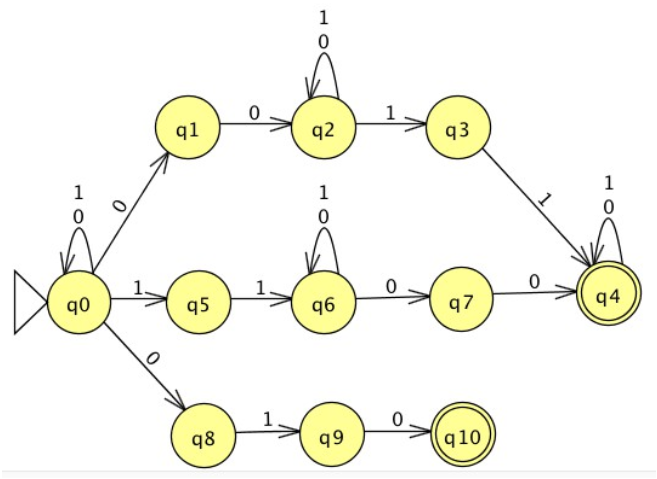
\includegraphics[scale=0.34]{q3_1}\newline
    \textbf{Construct} a DFA that recognizes all strings over $\{0, 1\}$ that contain 010 as a substring and does not end with 11.\newline
    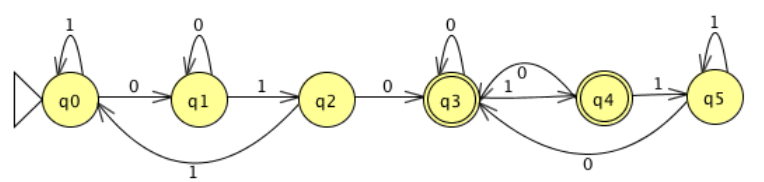
\includegraphics[scale=0.4]{q4_1}\newline
    \textbf{Construct} a CFG for $\{a^nb^md^ue^vc^k\mid v > 0; n, m, u, k\geq 0 $ and $n=m-k\}$\newline
    Since $n=m-k$ is equivalent to $m=n+k$, re-write as $a^nb^{n+k}d^ue^vc^k$ and then $(a^nb^n)(b^{k}d^ue^vc^k)$\newline
    $S\rightarrow AB$; $A\rightarrow aAb\mid \epsilon$; $B\rightarrow bBc\mid C$; $C\rightarrow dC\mid Ce\mid e$.\newline
    \textbf{Let} $L=\{w\mid w$ is an element of $\{a,b\}^*$ such that the number of a's in $w<$ the number of b's in $w<$ twice the number of a's in $w\}$\newline
    The basic idea is to mark an $a$ and then mark a corresponding $b$, if we run out of $a$s prior to $b$s we know that the number of $a$'s $<$ the number of $b$'s. We then start marking marked $a$s and corresponding $b$s. If we run out of $b$s prior to marked $a$s, then we know that the number of $b$'s $<$ twice the number of $a$'s.\newline
    \textbf{Let} $A$ be TR, $B$ decidable, $C$ can be enumerated in three weeks, 2 days, and 18 hours. $D$ is a TM that takes a TM $M$ and input $w$ and $M$ either halts within $2w$ transitions or $M$ never halts. $E$ is a CFL and $F$ a RL.\newline
    $C$ is context free since it is finite therefore a RL and therefor CFL.\newline
    $A\cap B$ is not decidable since $A$ intersected with $\Sigma^*$ is just $A$ and $A$ is only TR.\newline
    The compliment of $C$ is decidable as it is finite, it is a RL and it's compliment as well.\newline
    $D$ is decidable\newline
    $A\cap F$ is TR but not co-Turing recognizable.\newline
    Not all proper subsets of $B$ is decidable, consider $\{0,1\}*$\newline
    $E$ is a CFL, is decidable, and therefore co-Turing Recognizable.\newline
    The strings of $E$ having prime length is decidable.\newline
    The compliment of $F$ is decidable since $F$ is a RL.\newline
    \textbf{Let} $A$ be a decidable language and define $A'$ to be the collection of strings that are not in $A$, but contain a substring that is in $A$. Show $A'$ is also decidable.\newline
    Let $M$ be a TM that decides $A$. On input $w$, $X$ does:\newline
    (1) Run $M$ on $w$, if it accepts, then halt and reject\newline
    (2) For each substring $w'$ of $w$:\newline
    \indent(a) Run $M$ on $w'$ if accepts, then halt and accept\newline
    (3) Halt and Reject.\newline
    Since $M$ is a decider and we only run $M$ on a finite number of strings, we know $X$ will halt on all inputs. Claim $L(X) = A'$.\newline
    Let $w$ be an element of $A'$. Then $w$ is not in $A$, but $w$ has a substring that is in $A$. Step 1 verifies that $w$ is not in $A$ and step 2 verifies that $w$ contains a substring that is in $A$. By step 2, we accept $w$ thus $w$ is also an element of $L(X)$ and $A'\leq L(X)$.\newline
    Let $w$ be an element of $L(X)$. $w$ must be accepted in step 2, which means it contains a substring that is accepted by $M$. Thus $w$ has a substring in $A$. $M$ must also reject $w$ thus $w$ is not an element of $A$. By the definition of $A'$, $w$ is an element of $A'$ and $L(X)\leq A'$.\newline
    Therefore $L(X)=A'$ and $X$ decides $A'$ thus $A'$ is decidable.\newline
    \textbf{Let} $A$ be decidable, $C$ TR, and $D$ not TR. $B$ is just some language.\newline
    $A\leq_m B$ implies nothing about $B$ as $A$ is decidable.\newline
    $B\leq_m A$ implies $B$ is decidable therefore TR.\newline
    $B'\leq_m A$ then $B'$ is decidable and $B$ is TR.\newline
    $B \& B' \leq_m C$ then $B \& B'$ is TR and $B$ is decidable.\newline
    $B\leq_m C'$ implies nothing about $B$\newline
    $A\leq_mC\&C'$ implies nothing about $C$ or $C'$\newline
    $D\leq_m B$ implies $B$ is not decidable\newline
    $C'\leq_m C$ implies $C'$ is TR and therefore $C$ is decidable.\newline
    \textbf{Let} $A=\{\langle M \rangle \mid $ M is a TM and $L(M)$ contains at least two strings of odd length$\}$. Is it decidable?\newline
    No, $A$ is not decidable. Let $M$ and $M'$ be TM such that $L(M)=\{0,000\}$ and $L(M')=\{0\}$. Then $\langle M \rangle$ is in $A$ and $\langle M' \rangle$ is not in $A$, and the property of having at least two strings of odd length is non-trivial. Thus bu Rice's theorem $A$ is not decidable.\newline
    \textbf{Let} $A$ be a TR language, $B$ a co-TR language, $C$ a decidable language, and $D$ a language that can be enumerated in two years.\newline
    (TRUE) If $A$ and $B$ are the same language, then $A$ is decidable.\newline
    (FALSE) $B$ interset $C$ is decidable. If $C=\Sigma^*$ then $B\cap C = B$ so no reason to expect to be decidable.\newline
    (TRUE) $D^*$ concatenated with $C$ is decidable. $D$ is finite, so it is a RL which means $D^*$ is a RL and therefore decidable and closed under concatenation.\newline
    (FALSE) Any subset of $D^*$ is decidable. If $D=\{0,1\}$, then $D^*=\{0,1\}^*$ and $\{0,1\}^*$ has non TR subsets.
\end{multicols*}

\end{document}